\section{Motivation}
\label{sec:motivation}

\RED{Need a leading paragraph.}

\subsection{Total Store Ordering}
\label{subsec:tso}

\RED{Rewrite the following text in this subsection.}

We first list three categories of ordering anomalies that may take place in distributed systems with an asynchronous network.

\textbf{Send after write (SAW)}. A write data to shared storage X, then send a message to B, then B read the shared storage X, but find nothing. Figure~\ref{fig:causality} shows an example.

\textbf{Write after write (WAW)}. A write data to shared storage X, then write a metadata to shared storage Y. Asynchronously, B read the metadata from Y, then fetch the data from X, but find nothing.

\textbf{Independent read, independent write (IRIW)}. Initially, X=Y=0. A write to shared storage X=1 and B independently write to shared storage Y=1. C reads X=1, then reads Y=0; but D reads Y=1, then reads X=0.

In distributed systems without consistency guarantee, to remove RAW and WAW hazards, A needs to wait for the first write/read operation to finish until issuing the next operation, therefore limiting the concurrency. To remove IRIW hazards, the application needs timestamp, locking or explicit communication.

In latest x86 architecture, CPU cores issue memory access commands concurrently, but ensures a **total store ordering** memory model that ensures each core observe a consistent ordering of writes from all other cores. Logically, each CPU core maintains a cache of objects, and all cores share a FIFO of write operations. We extend the concept of total store ordering to distributed systems. Logically, the network resembles a FIFO and each end host receives messages in consistent ordering. More concretely, each message is assigned a monotonically increasing timestamp and each receiver receives messages in strict timestamp order (break ties by sender ID). If each read and write operation is transmitted as a unicast message in a FIFO network, we can validate that all three hazards are not possible.

In a distributed shared memory system, if the remote memory accesses are transferred via \sys, then all remote memory accesses obey total store ordering, similar to x86 multi-core memory consistency model~\cite{sewell2010x86}. Improved memory consistency can greatly simplify distributed coordination in distributed shared memory~\cite{sewell2010x86}.
 $A$ first issues write to a shared object $O$, then sends a message to $B$. When $B$ receives the message, it issues read from $D$. Due to variable network delay, $B$ may read the old value of $O$, violating causality. In a traditional distributed system, $A$ must wait for the write operation to complete before notifying $B$, introducing additional delay. If all the messages are sent via \sys, the read operation is guaranteed to have a higher timestamp than the write operation, so $B$ is guaranteed to read the updated value of $O$.





%\subsection{Total-Order Message Scattering}
%\label{sec:toms}

\iffalse
\begin{figure}[t]
\centering
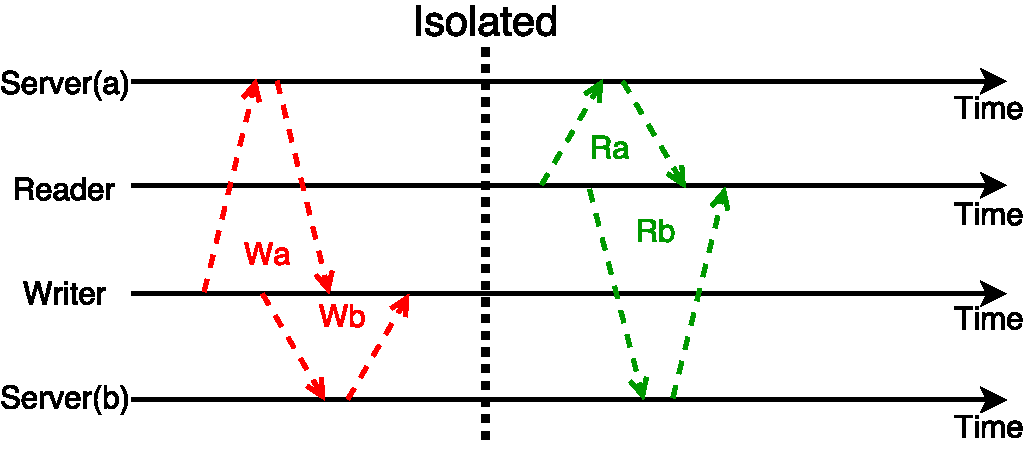
\includegraphics[width=0.48\textwidth]{images/read_write_isolation.pdf}
\caption{Two senders issue read and write requests to two receivers.}
\label{fig:example}
\end{figure}



\begin{figure}[t]
\centering
	\subfloat[Lock-based.\label{fig:concurrency-lock}]
	{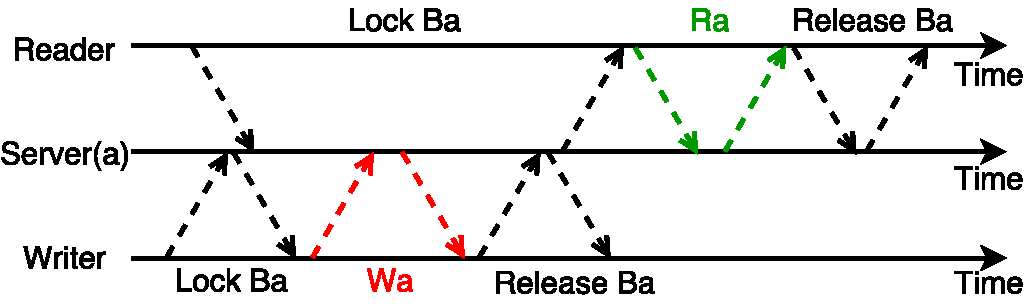
\includegraphics[width=.45\textwidth]{images/LockBased.pdf}}
    \hspace{0in}
	\subfloat[Timestamp-based (OCC).\label{fig:concurrency-timestamp}]
	{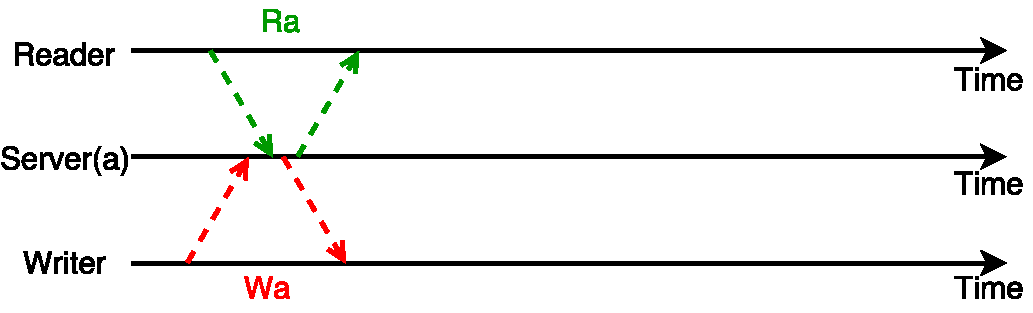
\includegraphics[width=.45\textwidth]{images/TimestampBased.pdf}}
	\caption{Two concurrency control mechanisms for distributed transactions.}
	\label{fig:concurrency-control}
\end{figure}
\fi


\begin{figure}[t]
\centering
	\subfloat[Possible causality violation due to variable network delay.\label{fig:causality_traditional}]
	{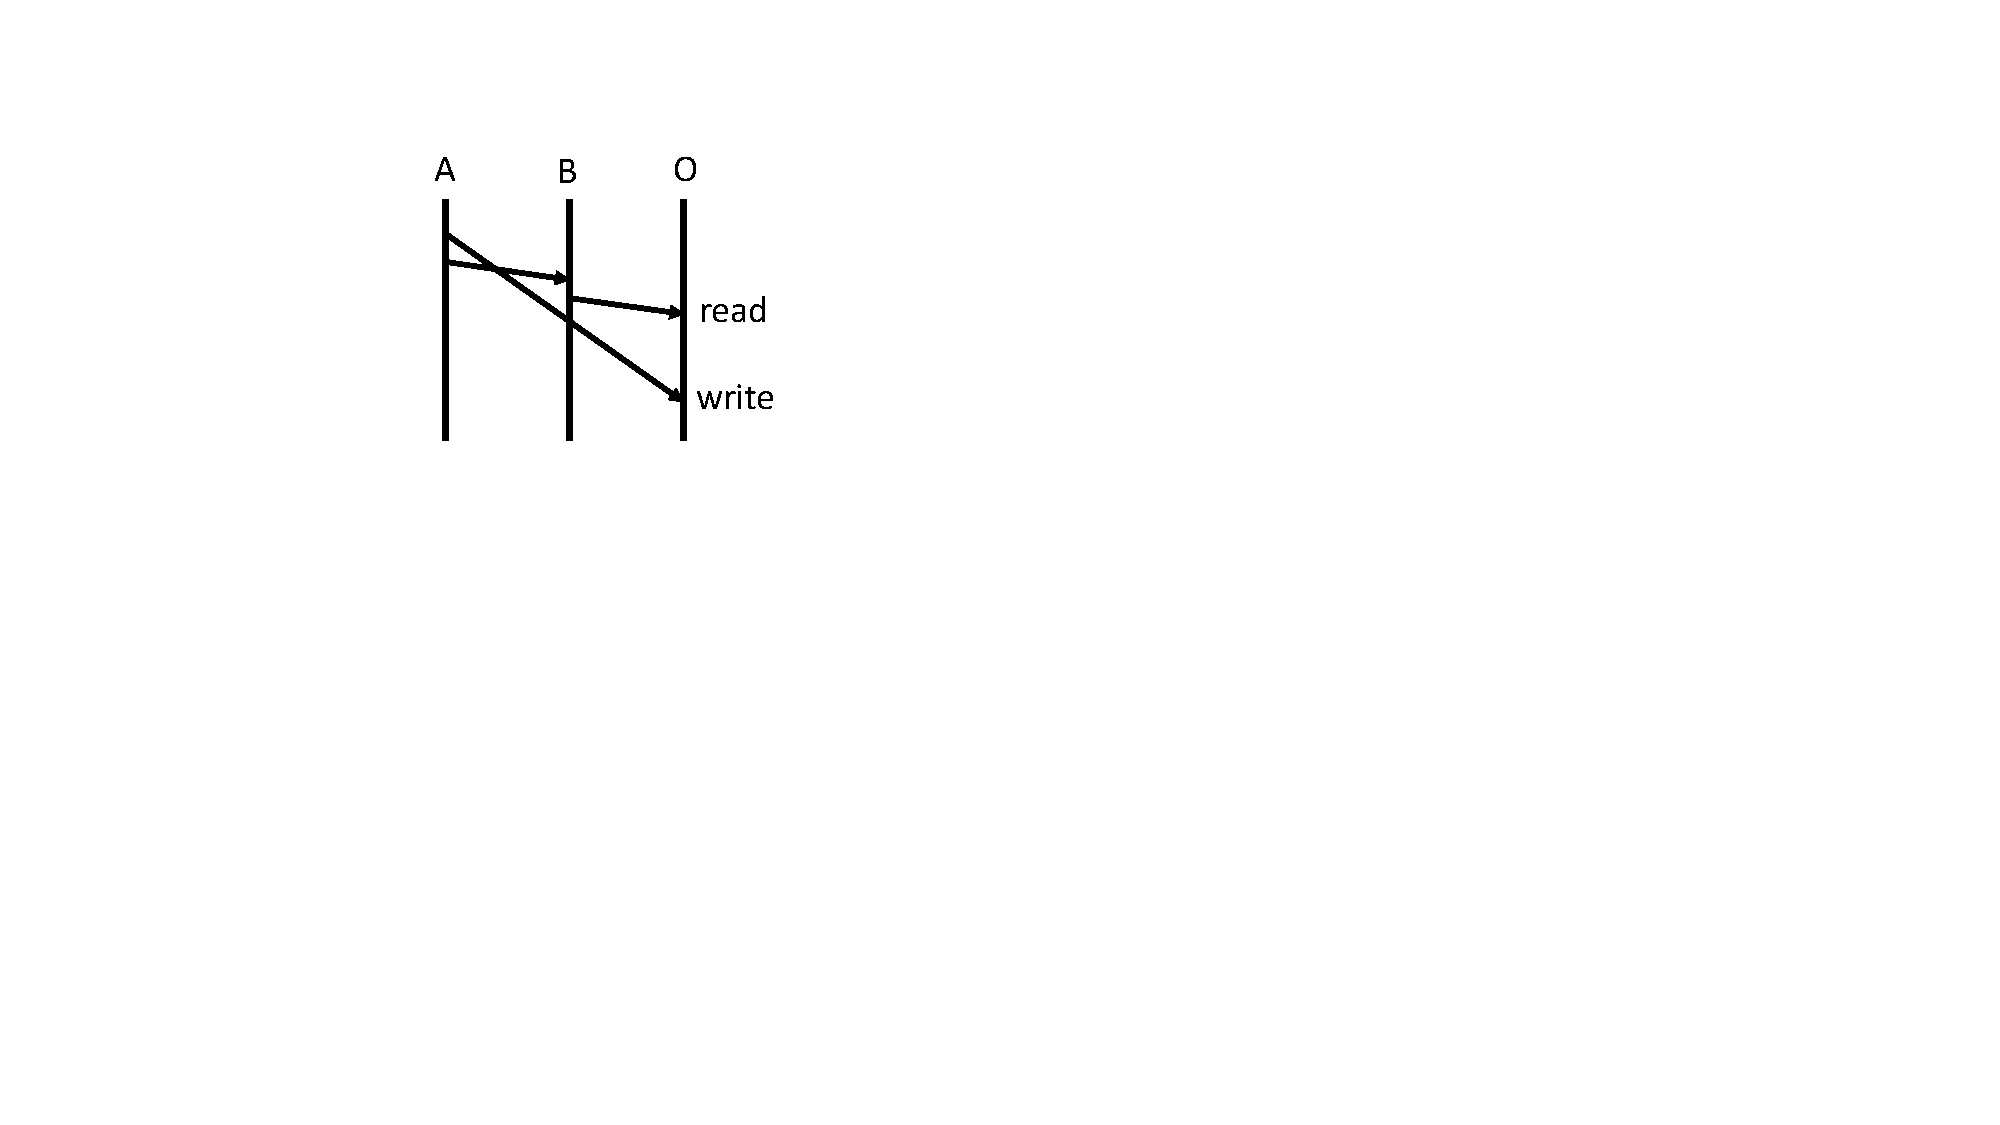
\includegraphics[width=.2\textwidth,page=1]{images/cropped_causality.pdf}}
    \hspace{0.03\textwidth}
	\subfloat[Guaranteed causality in \sys.]
	{\includegraphics[width=.2\textwidth,page=2]{images/cropped_causality.pdf}}
	\caption{Causality example: $A$ write shared object $O$, then notify $B$, then $B$ read $O$.}
	\label{fig:causality}
	\vspace{-1.5em}
\end{figure}


%The story begins with a hypothetical distributed banking system. Two accounts Alice and Bob are stored in different \textit{shards} at distant locations. Initially, their balances are $B_a$ and $B_b$. When Alice transfers \$1 to Bob, two write operations are sent to the shards: $B_a -= 1$ and $B_b += 1$, call them $W_a$ and $W_b$. At the same time, an auditor checks the total balance in the bank by accumulating balances of all accounts, resulting in two read operations: $R_a$ and $R_b$.
%If the system does not support transactions, the ordering of events may be $W_a < R_a < R_b < W_b$, then the auditor would find an inconsistent total balance.

%It is worth noting that \sys ensures ordering instead of consensus. When some hosts experience failure, \sys does not ensure a quorum of hosts agree on its received messages. NOPaxos~\cite{li2016just} has shown that \sys leads to an efficient implementation of distributed consensus.


\subsection{Transactional key-value store}
\label{subsec:transactional-kvs}

We will use a hypothetical banking example to illustrate the main concepts. Two accounts Alice and Bob are stored in different \textit{shards} at distant locations. Initially, their balances are $B_a$ and $B_b$. When Alice transfers \$1 to Bob, two write operations are sent to the shards: $B_a -= 1$ and $B_b += 1$, call them $W_a$ and $W_b$. At the same time, an auditor checks the total balance in the bank by accumulating balances of all accounts, resulting in two read operations: $R_a$ and $R_b$. If the system does not support transactions, the ordering of events may be $W_a < R_a < R_b < W_b$, then the auditor would find an inconsistent total balance.

A strongly consistent distributed system requires the reads and writes to be \textit{transactional}. The transaction $R_a, R_b$ and the transaction $W_a, W_b$ need to be performed in isolation.

There are two main categories of concurrency control to implement a transactional system. One category uses \textit{locks} to protect accesses to shared resources. The read transaction needs to lock $B_a$ and $B_b$, and the write transaction also needs to lock them. The transaction throughput is bounded by the \textit{round-trip time} (RTT) between the clients and the shards, because the lock must be sent from the shard to the client, then the client may send unlock to the shard.
In our example scenario where all transactions need to lock a single resource, if the RTT is 100~$\mu$s, the throughput is bounded to 10K transactions per second.

The other category is \textit{optimistic concurrency control} (OCC). It assigns a \textit{timestamp} to each transaction ($T_R$ for read, $T_W$ for write) and tracks object accesses during transaction execution. Transactions are serialized according to timestamp order. Once the system detects a \textit{late write}, that is, the write operation has lower timestamp than a read operation ($T_W < T_R$) but arrives later ($R_a < W_a$ or $R_b < W_b$), one of the transactions needs to be aborted and retried with a higher timestamp.
%Due to variable delays between clients and shards, if the read and write transactions are initiated at almost the same time, there are many possible orderings of $R_a, R_b, W_a, W_b$ and $T_R, T_W$. 
If the network delays between clients and shards follow a normal distribution, for two conflicting concurrent transactions, the probability of aborting one transaction is 3/4 with two shards. If each transaction involves $N$ shards, the abort probability is $1-(\frac{1}{2})^N$.

%If we regard each transaction as an event on a client, then the \textit{event timestamp} is the transaction timestamp. The read and write operations are the effects of the events, which propagate to the shards via messages.
%Each event may \textit{scatter} a set of messages to receivers (shards in our example). Each message is tagged with the event timestamp. Different messages may be scattered to different receivers, so \textit{broadcast} is a special case of \textit{scatter}.

To implement OCC without transaction aborts, we propose \textit{total-order message scattering} (\sys). \sys assigns timestamps to events and scatters messages from events, so that each host delivers messages to applications in monotonically increasing timestamp order (break ties by sender ID).
\sys provides a total ordering of all events in a distributed system, and ensures that each node observes the events (via messages) consistent with the total ordering.
With \sys, we regard each single-round-trip transaction as an event on the transaction initiator. In the absence of failure, transaction abort in OCC will never be triggered, because the read and write operations are always received by shards in the same ordering according to transaction timestamps.

\RED{Rewrite the following text in this subsection.}

If either read or write operations can tolerate end-to-end propagation delay of the whole network, TOMS can actually offer sequential consistency. We leverage this property to build a transactional key-value store, supporting multi-key atomic read and write operations.

Transactional key-value store requires more than total store ordering (sec. 2.1). First, atomic operations. When we use key-value store as a building block of more complicated data structures, we need to wrap multiple key-value operations in a critical section which execute atomically against other operations. \RED{Discuss scattering here.} Another use case of atomic operations is serializing updates. Each operation generates an output log and an error log. We hope that operations appear in consistent order in the output log and error log.

Second, reliable delivery. If a packet is lost in transactional key-value store, conflicting operations will be executed.

%In the distributed system, multiple \textit{hosts} are connected via the network. %A distributed system is made up of multiple \textit{hosts} connected via network. 
%An \textit{event} occurs on a host, and scatters messages to other hosts. For example, a distributed single-round-trip transaction can be regarded as an event on the transaction initiator, and its read and write operations are sent to the shards where the objects are stored. Here we use the term \textit{scatter} instead of \textit{multicast} because each shard only needs to receive operations related to the objects it host.


\subsection{Log serialization for geo-replication}
\label{subsec:log-serialization}

Recent years there is rich literature on improving eventual consistency in geographically replicated systems (COPS, Eiger, RedBlue...). The CAP theorem suggests that sequential consistency is not possible if both read and write operations have latency lower than inter-datacenter delay.

COPS and Eiger provide causal+ consistency in geo-replicated systems by tracking dependency of values or operations at shared storage servers. Causal consistency rules out WAW hazard. To rule out SAW hazard, message passing needs to be taken into account when tracking potential causal dependencies. Although causal+ ensures per-key sequential consistency by serializing the update log of each key, in the IRIW case, the change order observed by C and D may eventually diverge, because A and B are different keys. Furthermore, eventually consistent systems typically do not provide a bounded delay of convergence.

We build each replica as a transactional key-value store, and deploy another instance of reliable TOMS for replication traffic. TOMS serializes updates from all remote replicas. Applying the last-writer-wins rule on the timestamps of local objects and remote updates, the system will be eventually consistent, without the need of tracking causal dependencies or a convergent conflict handling function. TOMS also provides bounded convergence delay. After receiving replication at timestamp T and resolving conflicts, we are sure that the history before T will never be changed. Furthermore, we no longer need to replicate to all replicas to ensure total ordering of updates (cite The Potential Dangers of Causal Consistency and an Explicit Solution, SOCC'12).
